\chapter{Results} % Main chapter title
\noindent\textbf{\large Contents:}

\noindent\hrulefill
\noindent\startcontents[chapters]
\noindent\printcontents[chapters]{}{1}{}
\noindent\hrulefill
\label{Chapter4}

% \begin{itemize}
%     \item Cross-talk and detection region
%     \item analysis
%     \item conclusion and future work
% \end{itemize}

This chapter will go over the results of the simulation work as well as results from the optical testbed.

\section{Simulation Results}
\label{sec:sim}

With the control matrix in place, there needs to be data showing that there is a good linear correlation between the amplitude of the input wavefront aberration and what the system outputs.  Going through the process used in \S \ref{sec:RM}, a new set of aberrations were made with a range of amplitudes.   Then following the process described at the end of \S \ref{sec:CM}, we can compare the input amplitudes and what the code detects.  

\begin{figure}[H]
    \centering
    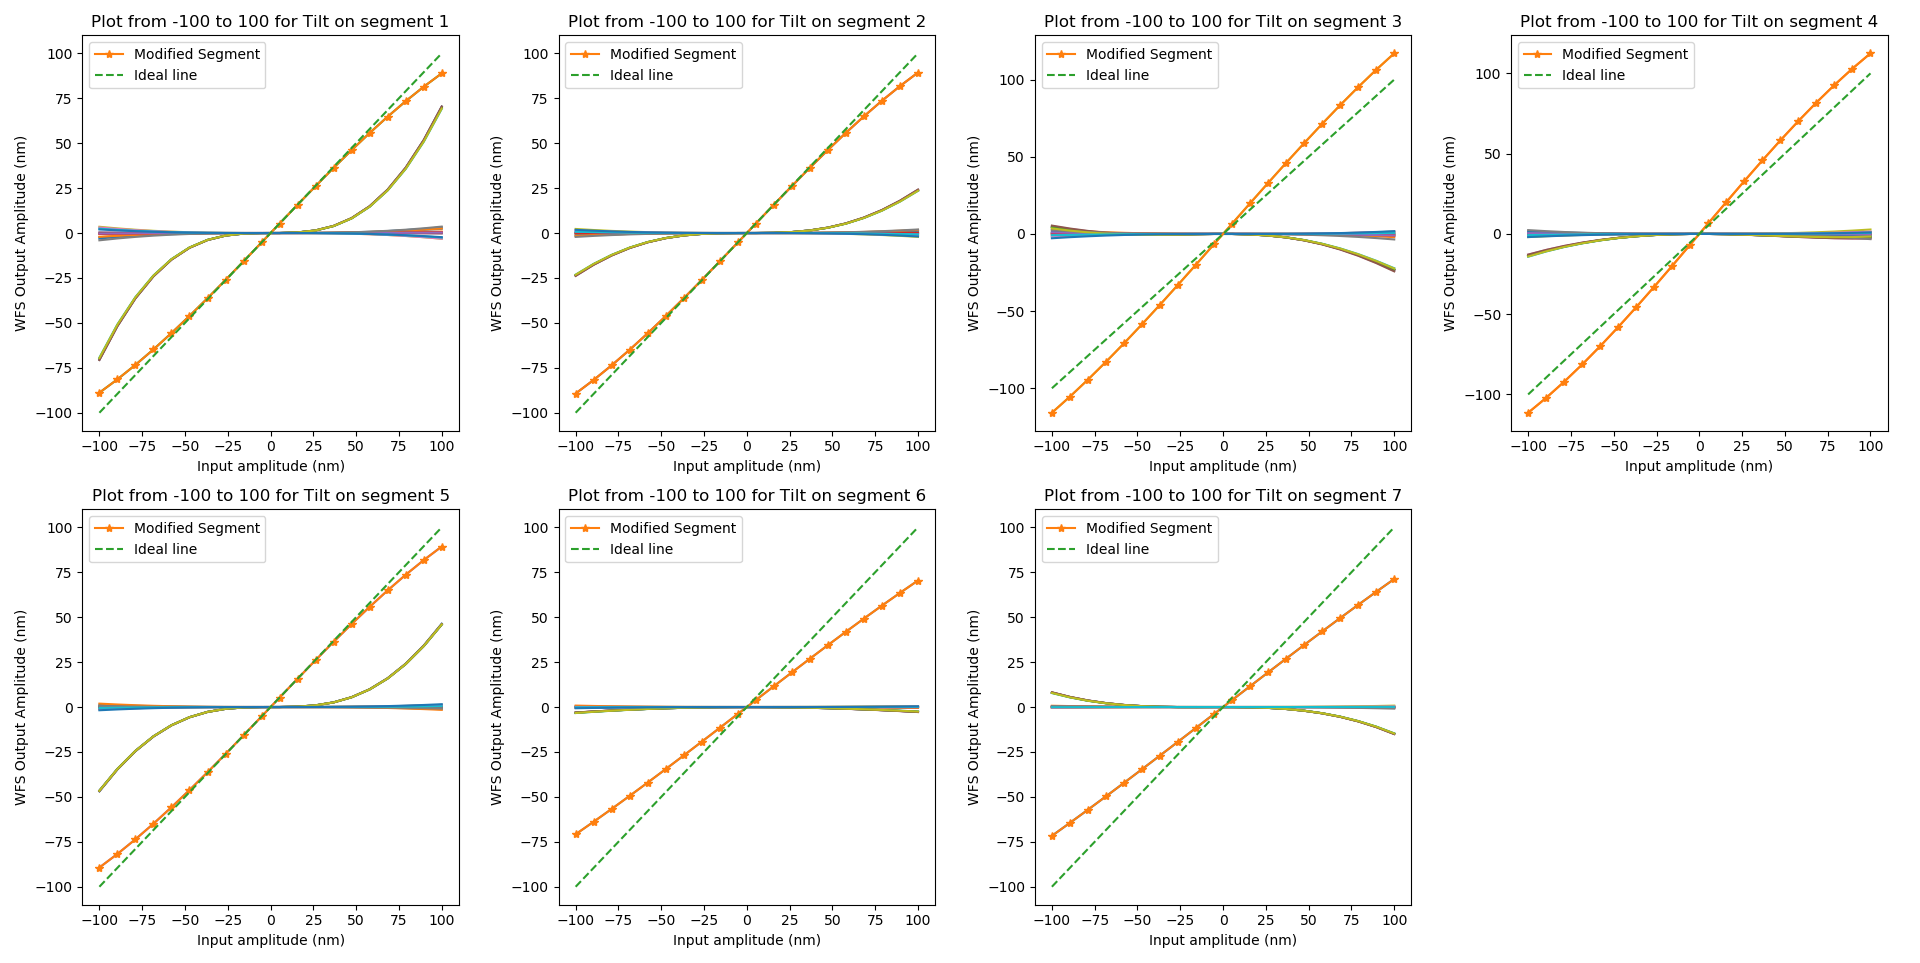
\includegraphics[width = 14cm]{Figures/Tilt_response100.png}
    \caption{Plots of each segments correlation between input aberration amplitudes and the output.  There are 21 lines for each mode in the modal basis set.}
    \label{fig:Tilt_100}
\end{figure}

As an example we will focus on the tilt of each segment.  As we can see in Figure \ref{fig:Tilt_100}, there is a linear region in the middle of each segment.  There is also some response from other modes.  This is cross-talk between other tilt modes from other segments.  However there is a region in the middle where cross-talk is limited.  Therefore the code ran again at to see the where the linear region lies.

\begin{figure}
    \centering
    \includegraphics{}
    \caption{Caption}
    \label{fig:my_label}
\end{figure}

\section{Testbed Results}
\label{sec:testbed}


\section{Future Work}
\label{sec:future}